\documentclass[a4paper,12pt]{article}
\usepackage[osf]{mathpazo}
\usepackage{ms}
\usepackage[numbers, sort&compress]{natbib}
\usepackage{lineno}
\usepackage{graphicx}
\usepackage{caption}
\modulolinenumbers[5]
\linenumbers

\pdfminorversion=3

\makeatletter
\renewcommand{\@biblabel}[1]{\quad#1.}
\makeatother

\title{The adequacy of phylogenetic trait models}
\author{
Matthew W. Pennell$^{1, *}$, Richard G. FitzJohn$^2$,\\
William K. Cornwell$^{3}$ \& Luke J. Harmon$^{1,4}$
}

\date{}
\affiliation{
 $^{1}$ Department of Biological Sciences \& Institute for Bioinformatics and Evolutionary Studies, University of Idaho, Moscow, ID 83844, U.S.A.\\ 
 $^{*}$ Email for correspondence: \texttt{mwpennell@gmail.com}\\
 $^{2}$ Department of Biological Sciences, Macquarie University, Sydney, NSW 2109, Australia;
\texttt{rich.fitzjohn@gmail.com}\\
 $^{3}$ School of Biological, Earth and Environmental Sciences, University of New South Wales, Sydney, NSW 2052, Australia; \texttt{w.cornwell@unsw.edu.au}\\
 $^{4}$ \texttt{lukeh@uidaho.edu}
}

\runninghead{are macroevolutionary models adequate?}
\keywords{comparative methods, model adequacy, independent contrasts, Brownian motion}


\begin{document}

\mstitlepage
\parindent=1.5em
\addtolength{\parskip}{.3em}
\vfill

\singlespacing
\section{Abstract}
Phylogenetic thinking is now pervasive in biology. Researchers from a variety of fields are increasingly using phylogenetic comparative methods (PCMs) to test evolutionary hypotheses using interspecific data.  PCMs requires both a phylogeny and a statistical model that describes the evolution of the trait through time.
A wide variety of such models have been proposed, all of which necessarily make
simplifying assumptions. In selecting a model, researchers have relied, almost exclusively, on measures of relative fit. Disconcertingly, we currently have no way of knowing if any of the models used in comparative biology provide good explanations for the data. Here we address two outstanding questions in comparative biology. First,
we develop a general framework for assessing the absolute fit (or, adequacy) of quantitative trait models, based on Felsenstein's Independent Contrasts method. Our framework can be applied to arbitrarily complex quantitative trait models. We then use our approach to assess whether commonly used models are reasonable descriptors of the macroevolutionary dynamics of three important angiosperm functional traits. We find that model fit is surprisingly poor; this is true across many clades and at multiple time scales. We argue that this result has serious implications for both developers of comparative methods and studies that make use of them. Assessment of model adequacy should become a routine component of phylogenetic comparative studies.

\vfill

\newpage



\begin{quotation}
\noindent There are known knowns; there are things we know we know. There are known unknowns; that is to say, there are things that we now know we don't know. But there are also unknown unknowns --- there are things we do not know we don't know.

---Fmr. U.S. Secretary of Defense Donald Rumsfeld
\end{quotation}

\section{Introduction}
Nothing in biology makes sense except in light of phylogeny. Long central to systematics and taxonomy, phylogenetic trees and phylogenetic thinking are ubiquitous in modern biology \citep{PennellHarmon}; ecologists, geneticists, paleontologists and anthropologists now widely recognize that a historical perspective can provide novel insights into evolutionary questions. This interest in phylogenetic biology has risen in lockstep with developments in phylogenetic comparative methods (PCMs) (reviewed in \citep{PennellHarmon}). Modern PCMs are almost exclusively model--based, meaning inferences are contigent on both the phylogenetic tree and the chosen probabilistic model. Selecting a good model is therefore essential for making robust inferences. Model choice should be guided by several considerations. One is interpretation: does the model capture the processes relevant to the question \citep{HansenOrzack2005, Hansen2012, PennellPE}? Another, the focus of this paper, is statistical: does the model provide a good explanation for the dataset? In phylogenetic comparative biology, this latter question has been addressed almost exclusively, by comparing the relative fit of a number of models and selecting the best one, by some criterion, for inference \citep{Mooers1999, Harmon2010, Hunt2012}. 

But the relative support for a model is only a partial answer to the question of whether it is a good explanation for the data. It is also important to consider whether the model is a good fit, or adequate, on its own terms. The best of a bad set of models is still a bad model. Assessing model adequacy is a routine step in many statistical applications, especially Bayesian statistics \citep{Gelmanbook}. Failure to check model adequacy can potentially result in erroneous inferences. A classic example of this in molecular systematics is the disputed phylogenetic relationships of rodents. A number of early molecular phylogenetic studies reported evidence that ``strongly contradict[ed]'' the traditional hypothesis that the order Rodentia is a monophyletic group (e.g., \citep{Graur1991, DErchia1996}). Sullivan and Swofford \citep{Sullivan1997} demonstrated that these conclusions were misleading, and resulted from using models of molecular evolution that did not adequately accomodate  heterogeneity in rates of evolution across sites. There are many similar case--studies throughout and outside of evolutionary biology.

Many models for describing the evolution of phenotypic traits along a phylogeny have been developed, as well as sophisticated machinery for fitting them to data (e.g., \citep{Felsenstein1985, Hansen1997, Pagel1999, Blomberg2003, ButlerKing2004, Omeara2006, Eastman2011, Beaulieu2012, SlaterMEE}). Using these models, researchers from across biology disciplines have made exciting discoveries that would not have been possible without a phylogenetic perspective. However, it is disconcerting that we generally have no idea if the models used in PCMs are adequate. There are no general procedures that can be used to assess the adequacy of all of the models referenced above. Even more troubling is that model adequacy is rarely ever considered when PCMs are applied. To borrow Rumsfeld's taxonomy, model adequacy has largely been an ``unknown unknown'' in PCMs.

In this paper we seek to (at least somewhat) rectify this situation. We address two major outstanding problems in comparative biology. First, we develop a general framework for assessing the adequacy of phylogenetic models of trait change, specifically those for quantitative characters. Second, we assess the adequacy of simple models of trait evolution across scales, using a recently published mega--phylogeny of Angiosperms (flowering plants) \citep{Zanne2013} and data on three important functional traits --- specific leaf area, seed mass, and leaf nitrogen content --- compiled from the literature. We find that in this dataset, commmonly used models of character evolution have woefully poor adequacy. And the adequacy becomes increasingly worse with larger datasets. To what extent this result generalizes to other datasets is not known, but our results raise very serious concerns about current practices in comparative biology.

\section{A general framework for assessing model adequacy}
The basic concept of our approach is straightforward. We have a phylogenetic tree consisting of $n$ lineages. We have data on the the trait values observed at each tip $X = X_1, X_2, \ldots, X_n$. In order to make inferences from the distribution of traits at the tips, we fit a model $\mathcal{M}$ describing the evolution of the trait along the phylogeny. In most analyses using comparative data, the aim is to ask: what $\mathcal{M}$ maximizes the likelihood of observing $X$?; what is the posterior distribution of $\mathcal{M}$?; or, does $\mathcal{M}_1$ better explain the data than $\mathcal{M}_0$? Our approach is conceptually distinct in that we are trying to ask: how likely is it that $\mathcal{M}$ would produce a dataset similar to $X$ if we re--ran evolution?

We have developed two separate ways to ask this question --- one frequentist, the other Bayesian. While these approaches are philosophically different from one another, in practice, they are very similar. In a frequentist paradigm, we can assess model adequacy by performing parametric bootstrapping. We estimate $\mathcal{M}$ using maximum likelihood, restricted maximum likelihood, least--squares, etc. We then simulate new datasets $Y$ by evolving a trait along the phylogeny according to $\mathcal{M}$. We can then compare $X$ and $Y$. However, In order to make any sort of comparison, we must first summarize $X$ and $Y$ using a meaningful summary statistic or a set of summary statistics $\mathcal{S}$. If $\mathcal{S}_X$ is more extreme than most of the distribution of $\mathcal{S}_Y$, we can conclude that $\mathcal{M}$ is not a good explanation for $X$. Parametric bootstrapping procedures are likely familiar to phylogenetic biologists in the form of the Goldman--Cox test \citep{Goldman1993} for the adequacy of sequence evolution models, and the Shimodaira--Hasegawa (SH) \citep{SH} test for comparing topologies. Recently, Boettiger et al. \citep{Boettiger2012} used a Monte Carlo procedure to assess the fit of comparative models, though with some important distinctions from our approach (see below).

Alternatively, one may adopt a Bayesian perspective and estimate the posterior distribution of $\mathcal{M}$, $\mathbb{P}(\mathcal{M}|X)$ using Bayes theorem
\[\mathbb{P}(\mathcal{M}|X) = \frac{\mathbb{P}(X|\mathcal{M})\mathbb{P}(\mathcal{M})}{\mathbb{P}(X)} \]
and Markov chain Monte Carlo (MCMC machinery). To assess the adequacy of the model we perform posterior predictive simulations \citep{Rubin1984, Gelman1996}. The posterior predictive distribution
\[\mathbb{P}(Y|X,\mathcal{M}) = \int \mathbb{P}(Y|\mathcal{M})\mathbb{P}(\mathcal{M}|X)d\mathcal{M}. \]
$\mathbb{P}(Y|X,\mathcal{M})$ is simply the probability of getting a new dataset $Y$ given $X$ and $\mathcal{M}$. We obtain this distribution by drawing repeated samples from $\mathbb{P}(\mathcal{M}|X)$ and simulating datasets from the sampled parameters. [more] Posterior predictive simulation appraoches have also been developed for molecular phylogenetics \citep{Bollback2002, Reid2013, Lewis2013, Brown2013} but have unfortunately not been widely adopted \citep{Brown2013}.


\subsection{Summary statistics}
As stated above, in order to compare the observed data $X$ with the data simulated under the fitted model $Y$ we need some way of summarizing the observations to make meaningful comparisons. 
In our approach we calculate a set of summary statistics on the contrasts (\textit{sensu} Felsenstein \citep{Felsenstein1985}) computed at each node, rather than on the data itself. (We refer readers to \citep{Felsenstein1985, Rohlf2001, Blomberg2012}, for details on how contrasts are calculated.) Contrasts are a natural way of summarizing phylogenetically structured quantiative data with very little loss of information (i.e., only lose 1 degree of freedom). Importantly, contrasts have the useful statistical property that if BM is a good model for the evolution of the trait, they will be independent and identically distributed (i.i.d.) $\sim \mathcal{N}(0, \sigma)$. The raw data can only be i.i.d. if the phylogeny is not informative. 

We have chosen a set of six summary statistics $\mathcal{S} = \lbrace \mathcal{S}_1, \ldots, \mathcal{S}_6 \rbrace$ to compute on the contrasts of both our observed data and our simulated data.

\begin{enumerate}
\item[$\mathcal{S}_1$] The mean of the squared contrasts. This is equivalent to the restricted maximum likelihood (REML) estimator of the Brownian motion rate parameter $\sigma^2$ \citep{Garland1992, Rohlf2001}. $\mathcal{S}_1$ is a used as a global rate estimate.

\item[$\mathcal{S}_2$] The variance in the absolute value of the contrasts. If the variance of the observed contrasts is greater than that of the simulated contrasts, it suggests that we are not properly accounting for rate heterogeneity across the phylogeny. If the variance of the observed is smaller, it suggests that trait is somehow more contrained than the model assumes.

\item[$\mathcal{S}_3$] The slope resulting from fitting a linear model between the absolute value of the contrasts and their expected variances, with the expected variances as the independent variable. Each (standardized) contrast has an expected variance proportional to the sum of the branch lengths connecting the node at which it is computed to its daughter lineages  \citep{Felsenstein1985}. Under a model of BM, we expect no relationship between the contrasts and their variances. We use $\mathcal{S}_3$ to test if contrasts are larger or smaller than we expect based on their branch lengths. If, for example, more evolution occured per unit time on short branches than long branches, we would observe a negative slope.

\item[$\mathcal{S}_4$] The slope resulting from fitting a linear model between the absolute value of the contrasts and the inferred ancestral state, with the inferred ancestral states as the independent variable. We estimated the ancestral state using the least--squares method suggested by \citep{Felsenstein1985} for the calculation of contrasts. We note that this is not technically an ancestral state reconstruction (it is more properly thought of as a weighted average value) and differs from more commonly applied approaches, such as the  maximum likelihood estimator \citep{Schluter1997}. We used this statistic to evaluate whether there is variation in rates relative to the trait value (e.g., do larger organisms evolve proportionally faster than smaller ones?)

\item[$\mathcal{S}_5$] The slope resulting from fitting a linear model between the absolute value of the contrasts and the height of the node at which they are inferred measured from the root, with the node height as the independent variable. For $\mathcal{S}_5$, we used the original node heights rather than the transformed node heights obtained from calculating the contrasts. This is used to capture variation relative to time and is alternatively known as the ``node--height test'' \citep{FreckletonHarvey2006, SlaterPennell} for detecting early bursts of trait evolution in putative adaptive radiations. It has been  previously used to assess the fit of BM models.

\item[$\mathcal{S}_6$] The D--statistic obtained from Kolmolgorov--Smirnov test from comparing the distribution of contrasts to that of a normal distribution with mean 0 and standard deviation equal to the root of the mean of squared contrasts (the expected distribution of the contrasts under BM; see \citep{Felsenstein1985, Rohlf2001}). We chose this to capture deviations from normality. For example, if traits evolved via a ``jump--diffusion'' type process \citep{Landis2012}, in which there were occasional large ``jumps'' in phenotypic space \citep{PennellPE}, the tip data would no longer be multivariate normal owing to a few contrasts throughout the tree being much larger than the rest. 

\end{enumerate}

The three summary statistics fitting a linear model between the contrasts and some aspect of the data (i.e., $\mathcal{S}_3$, $\mathcal{S}_4$, and $\mathcal{S}_5$) were developed by Garland and colleagues \citep{Garland1992, Garland1993,  Diaz1996} to test for adequacy of BM prior to performing PIC \citep{Felsenstein1985} or phylogenetic regression \citep{Grafen1989} tests for the evolutionary correlation between traits. 

We have chosen these six summary statistics because they capture a range of dimensions of variability wherein the model may not be adequate. However, they are certainly not exhaustive. One could, for instance, calculate the median of the squared contrasts, the skew of the distribution of contrasts, etc. If the generating model was known, we could use established procedures for selecting a set of sufficient (or, approximately sufficient \citep{MajoramJoyce}) summary statistics for that model. However, the aim of our approach is assess the fit of the model without reference to a true model. Our chosen statistics capture a wide variety of model misspecifications but this does not mean that they will necessarily capture every type of model misspecification. Researchers interested in specific questions are encouraged to use alternate sets of summary statistics. The choice of what summary statistics to use is ultimately one of balancing statistical intuition and computational effort. Unfortunately, there is no good statistical theory to guide us as to which summary statistics to use and how many are enough \citep{Gelmanbook}.

\subsection*{Generalizing the approach}

All of the summary statistics we use essentially evaluate the condition that the contrasts are i.i.d. and come from a normal distribution. If we assume that the data has arisen as a result of a BM--like process and this condition does not hold, the model can be rejected as inadequate. Our summary statistics $\mathcal{S}_3$, $\mathcal{S}_4$, and $\mathcal{S}_5$ have been used previously in the literature with this justification (e.g., \citep{Garland1992, Garland1993,  Diaz1996}). However, if we assume that our traits have evolved under a different model, such as an OU or a multi--rate BM model, then we no longer necessarily expect the contrasts to be i.i.d. The expected distribution of contrasts under most models is not characterized and even if it was, this would necessitate a model--specific set of summary statistics for every model.

Our solution to this problem is to create what we term a ``unit tree'' (see Box 1). A unit tree is defined as a phylogeny which has branch lengths in units of (standardized) variance. We can rescale a phylogeny with branch lengths in time units (e.g., my) to a unit tree using the parameters of any quantitative trait model, as long as the data at the tips is assumed to come from a multivariate normal distribution. This applies to nearly all models used in comparative biology \citep{Omeara2012} (see \citep{Landis2012} for a notable exception). If the model that is fit is the generating model, or an adequate alternative, the contrasts will be i.i.d. according to a standard normal distribution $\mathcal{N}(0,1)$. In other words, if the model is good, the trait data at the tips will have the same distribution as data generated under a BM process with a rate of 1 (hence the term ``unit tree''). Creating the unit tree from the estimated model parameters prior to computing the contrasts generalizes the summary statistics to most models of trait evolution.

Calculating the contrasts on the unit tree also means that rather than simulate trait evolution under the model, we can simulate many datasets under a BM process ($\sigma^2 =$1), which is computationally efficient. The distribution of summary statistics calculated on these simulated data sets can then be compared to the summary statistics from the observed data. We summarize the entire approach in Figure \ref{fig:flowchart}.

\subsection{A case study: seed size evolution in the Meliaceae and Fagaceae }
%% TODO (MWP): check all numbers used in this section.
To illustrate our approach we examine seed size evolution in two tree families, the Meliaceae (the mahogany family) and Fagaceae (which contains oaks, chestnuts and beech trees). The trait data and phylogeny for both groups are subsets of the larger dataset used in the analysis (see below). Superficially, these datasets are quite similar. Both are of similar size (Meliaceae: 44 species in dataset; Fagaceae: 70 species) and are ecologically comparable. Following Harmon et al. \citep{Harmon2010} we fit three models of trait evolution to the data: BM, OU and an Early Burst (EB) model, in which the rate of evolution declines exponentially through time \citep{Blomberg2003, Harmon2010} (see below for details). We computed AIC weights \citep{aicweight} for the three models and for both datasets, an OU model was overwhelmingly supported (AICw $>$ 0.98 for both groups). Using the conventional model selection approach commonly used in comparative biology, we might conclude that similar evolutionary processes are important in these two clades of trees.

Examining model adequacy provides an alternative perspective. We took the MLE of the parameters from the OU models for each dataset, constructed a unit tree based on those parameters. We calculated our six summary statistics on the contrasts of the data, then simulated 1000 BM datasets on the unit tree and calculated the summary statistics on the contrasts of each simulated dataset. The results from the analyses of model adequacy are shown in Figure \ref{fig:two-clades}. For seed size evolution in Meliaceae, the OU model selected by AIC was an adequate model; the observed summary statistics were in the middle of the distribution of simulated summary statistics ($\mathcal{S}_1: p=0.448$, $\mathcal{S}_2: p=0.803$, $\mathcal{S}_3: p=0.633$, $\mathcal{S}_4:p=0.496$, $\mathcal{S}_5: p=0.148$, $\mathcal{S}_6: p=0.629$). For the Fagaceae, the story is different. The OU model was revealed to be inadequate by both $\mathcal{S}_1$ ($p \sim 0$) and by $\mathcal{S}_2$ ($p=0.006)$; the rest of the observed summary statistics did not differ significantly from the simulated summary statistics ($\mathcal{S}_3: p=0.228$, $\mathcal{S}_4:p=0.364$, $\mathcal{S}_5: p=0.828$, $\mathcal{S}_6: p=0.955$). This example serves to illustrate the distinction between the conventional approach to model selection in PCMs and model adequacy. Selecting amongst a limited pool of models does not give a complete picture of whether a model is appopriate. We will return to this case study in this discussion.


\section{The adequacy of models for the evolution of plant functional traits}

We used the approach we developed to address an outstanding question in comparative biology: how well do commonly used models explain the evolution of traits along a phylogeny and when are more complex models required. We addressed this question by studying Angiosperm functional traits using a recently published a megaphylogeny of containing 31,749 species of seed plants \citep{Zanne2013}. This dataset is exceptional in terms of scope and allowed us to evaluate the adequacy of models through time and across many groups.  

We compiled data on three traits from the literature --- specific leaf area (SLA), seed mass and nitrogen content (see Methods for details on datasets). These are commonly used proxies for functional variation in plants (e.g., hydrodynamic cycling, life history characteristics, and photsynthetic capabilities, respectively \citep{Westoby2002}). We  matched these data to the phylogeny. Following Harmon et al. \citep{Harmon2010} and pulled out xx subclades, extracting named (family and orders) and unnamed clades taken from time--slices across the tree. For each subclade, fit three simple models of trait evolution: 1) BM, which is often associated with genetic drift \citep{Lande1976, Felsenstein1988, Lynch1990, HansenMartins1996}, randomly--varying selection \citep{Felsenstein1973}, or the summation of many processes over macroevolutionary time \citep{HansenMartins1996, Uyeda2011, PennellPE}; 2) single optimum OU, which is often assumed to represent stabilizing selection (following Lande \citep{Lande1976}), though we think a more meaningful interpretation is that it represents an ``adaptive zone'' \citep{Arnold2001, Hansen2012book PennellHarmon}; and 3) EB, which was developed as a mathematical represenation of a niche--filling process during an adaptive radiation \citep{Harmon2010, SlaterPennell}. We evaluated the relative support for each of the three models using conventional model selection techniques and then assessed the adequacy of the models using our procedure. (See Methods section for further details.) 

\section{Results}

[RESULTS]

\section{Discussion}

Phylogenies are increasingly being recognized as essential data in evaluating macroevolutionary and macroecological hypotheses. However, as stated in the introduction, the phylogeny alone is not sufficient --- we also need a statistical model of trait evolution to describe the expected pattern of variation across the phylogeny. 

The patterns of trait evolution along a phylogeny has been shaped by numerous processes: selection and drift across an adaptive landscape; the dynamics of adaptive landscapes themselves; and potentially higher--level selection (i.e., species selection) on lineage--level traits \citep{PennellPE}. As biologists, we need to consider whether a given model allows us to gain insight into the evolutionary question of interest \citep{HansenOrzack2005, Hansen2012}. We also need to address the more statistical question of whether the model adequately captures the variation we are interested in. These two considerations --- biological and statistical --- must go hand--in--hand; a biologically informative model may be a poor fit to the data and a model that captures the variation in the data may not provide any biological insight \citep{Hansen2012}. In this paper, we focus on the statistical aspect of modeling trait evolution but emphasize that any model--fitting exercise is pointless unless guided by sound evolutionary thinking.

To date, comparative analyses have for the most part only considered a single model (such as BM) or else performed some sort of model comparison to select amongst a set of competing models. Whether or not the selected model is actually capturing the relevant patterns in the data --- that is, whether the model is adequate in the absolute sense -- has been largely overlooked and this may have very serious consequences for any inferences drawn from these analyses. Here we present a general framework for assessing the adequacy of phylogenetic models of continuous characters. Our approach can apply to any model in which the traits at the tips of the phylogeny are assumed to come from a multivariate normal distribution. Mechanically, our method is rather simple but we believe that it can be extremely useful for future analyses of comparative data. We argue that all phylogenetic comparative analyses should include a model--checking component; doing so will help ensure that the inferences obtained from them are reliable.

As we demonstate in our analysis of the evolution of plant functional traits, the simple models often used in comparative biology are often inadequate and woefully so at large scales. Our results should give researchers cause for serious concern. Though phylogenetic comparative analyses have been widely performed throughout the literature, there has not been any method for validating the model used. Our results suggest that many previous comparative analyses may need to be re--evaluated in light of model adequacy. The very tight scaling of model (in)adequacy with tree size suggests that concerns about model adequacy are especially pertinent when analyses are conducted on large phylogenies. Of course no biologist is likely to be shocked by our findings; indeed, one of the main reasons we are interested in studying macroevolutionary diversity is the complexity of the processes that may have generated it.  

\subsection{Model adequacy for angiosperm functional traits}
Major patterns we found.

\subsection*{Why models may be inadequate}
There are a number of likely interacting causes for model inadequacy. The most biologically interesting of these is that the evolutionary processes in some group are more complex (or just different) from the processes and patterns accounted for by our model.  There is substantial evidence from both phylogenetic comparative and paleobiological data than the patterns of evolution are often quite complex, with different processes and different rates occuring across the phylogenies of many groups \citep{Foote1997, Grey2008, Hunt2012, Hopkins2012, PennellPE}. It is likely that phylogenetic models of trait evolution which do not accomodate such variation are inadequate. In our analyses of plant functional trait evolution, we used only simple models of trait evolution. It is undoubtedly true that at the larger scales (and often at smaller ones), a single rate or single--optimum model is likely to be woefully inadequate for traits like seedmass \citep{Moles2005}. Thus, far from a nuisance, assessing model adequacy may tell us interesting things about the biology of a group which would not be apparent from solely comparing relative fits of a limited set of candidate models. There has been a lot of progress recently in the developement of more sophisticated and parameterized models of trait evolution \citep{ButlerKing2004, Omeara2006, FitzJohn2010, Eastman2011, Venditti2011, Revell2012, Beaulieu2012}. Our approach can help researchers decide when it is necessary to invoke further complexity. Importantly, knowing which summary statistics reject a model can provide insight into what type of complexity (i.e. heterogeneity in rates and/or models) is necessarily to include in order adequately capture the variation in the trait.

Model misspecification is not the only source of error when fitting trait models. Estimating parameters, especially under likelihood, is often non--trivial owing to identifiability issues in some regions of parameter space \citep{Ane2008, HoAne2012}. This issue is generally underexplored but is likely to important, especially for more parameter--rich models. The construction of the unit tree depends on the parameter estimates and our measure of model adequacy will therefore be influenced by their mis--estimation. Second, measurement error may have pathological effects regarding model adequacy and the effects may vary depending on the model used \citep{PennellPE}. In our empirical analyses we used a global estimate of standard error. Ideally, we would have used observations from individuals and estimated the error along with the model \citep{Ives2007, Felsenstein2008,  Hansen2012}, but this type of data was not available for many taxa in our datasets. 

Phylogenetic misestimation may also have an effect on the adequacy of a model. All of the statistical models of trait evolution assume that branch lengths are estimated without error, though in practice this is never actually the case. The influence of branch length error in PCMs is not really known and its effect will depend on whether the error is random or systematically biased. Misestimating topology may have very serious consequences for model adequacy in some types of analysis. For example, if species are paired with the incorrect species, traits of sister species may appear to be more dissimilar than they really are, leading to inflated contrasts and rate estimation close to the tips. In our empirical example, the ML tree we used (from \citep{Zanne2013}) is likely to have substantial topological errors owing to the scale of the data and the analytical shortcuts inherent in building a ``megaphylogeny'' \citep{Smith2009}. The error in the topology (which is especially large towards the tips) may be a a major contributor to the inadequacy of the simple models across the functional trait datasets. 
A model can be inadequate as a result of any of these and it is often challenging to distinguish the contribution of these in real datasets. Our approach cannot provide a clear reason why a model is inadequate, only indicate that it is.

\subsection*{An adequate model does not necessarily mean a good model}
Simply because a model cannot be rejected with our approach does not necessarily mean that the model itself is a good one. First one must consider whether there is enough statistical power to reject a model. The more contrasts in a dataset (i.e. the more taxa), the more power there is to detect deviances from the expected distribution. We observed a strong positive correlation between a multivariate measure of model (in)adequacy and the number of taxa in a group (see above, figure XX). While as we argue above, it is likely that the pattern of evolution is increasingly complex at larger scales, it is also possible that the simple models we used were on average equally inadequate at all scales and we simply had more power to detect this on larger trees. This explanation is supported by the fact that there is little correlation between the age of the clade and the adequacy of the model (see supp fig). The power to reject a given model is inversely related to the ability to find support for a model, using some form of model selection.

Both the original model fit and the simulations are both based on the observed tip values. These may or may not be representative of the states that have occured throughout the clade's history. In other words, a model may adequately capture variation in our observed tip values but may be misleading when making inferences about the evolutionary history of the trait. Incorporating fossil taxa has been shown to dramatically alter the estimated model parameters and the evolutionary inferences \citep{FF2006, Slater2012Fossil, SlaterMEE}. Likewise, if contemporary species are sampled in a non--random way, such that some trait values are over-- or under--represented \citep{Freckletoninaction}, the model may explain the data but the inferences from the model may be misled. 

\subsection*{Extensions of this approach}
The framework we present here can be extended in number of ways. First, we have only considered a limited set of summary statistics. We chose them because each of these has a clear statistical expectation and observed deviations from them have intuitive explanations. However, they are certainly a subset of all possible summary statistics that could be applied. One thing we did not consider, for example, is autocorrelation between neighboring contrasts \citep{Gittleman1990}. One could also potentially use alternative forms of the contrasts, such as contrasts considering within species variation \citep{Felsenstein2008}, or alternative ways of assessing the summary statistics, such as using robust regression in lieu of fitting standard linear models for the 3 summary statistics involving slope ($\mathcal{S}_3, \mathcal{S}_4, \mathcal{S}_5$) (see \citep{SlaterPennell}). There are undoubtedly more such summary statistics that creative researchers could potentially conceive of; some will be more appropriate than others for different questions.

The method we have described here can apply to any model of trait evolution which can be described by a multivariate normal distribution. That is, where the original tree can be transformed from the model fitted parameters to a unit tree. Our approach can therefore not be applied to other types of models, such as those which assume a fat--tailed distribution of trait change \citep{Landis2012} or state--dependent diversification models \citep{Bokma2008, FitzJohn2010}. Our approach is also not applicable to models of discrete character evolution, such as the Mk model \citep{Pagel1994} and other variants \citep{Felsenstein2012, Beaulieu2013}. However, for these types of traits, approaches that have been developed to the adequacy of sequence evolution models \citep{Bollback2002, Lewis2013} could potentially be employed. Developing and implementing such methods for discrete character models is an important area for future research as model adequacy is just as pertinent a consideration as for the continuous case \citep{ReadNee1995}. 

Another possibility which our approach suggests is that researchers could potentially use the summary statistics as a means to perform question--specific model selection. This is the essence of the ``node--height'' test for detecting early bursts of trait evolution \citep{FreckletonHarvey2006}. Slater and Pennell \citep{SlaterPennell} developed a fully Bayesian posterior predictive method for detecting such early bursts from comparative data. For some problem, one may be care a lot about whether the model is capturing the variance in some axis (or axes) and be less concerned about others. One could then use posterior predictive simulations and a well--chosen set of summary statistics to help guide model selection \citep{Bollback2002, Lewis2013}. One could also potentially use summary statistics to construct cost functions and select amongst models in a decision--theoretic framework \citep{Robert2007}. Such an approach has proven to be very useful in selecting between models of sequence evolution \citep{Minin2003, SullivanJoyce2005} but has not been previously considered in comparative methods.

\subsection{Concluding remarks}
While we describe this as a novel approach, much of it stems directly from earlier work in the field. In the 1980s and 1990s --- the time when phylogenetic comparative biology was just starting to emerge as a discipline --- much discussion surrounded the appropriateness of various methods and models \citep{Felsenstein1985, Felsenstein1988, HarveyPagel1991, Garland1992, Pagel1993, Diaz1996, Price1997, Garland1999, GarlandIves2000}. However, as phylogenetic approaches have become more widely accepted and applied in a wider variety of fields, including community ecology \citep{Webb2002, CB2009}, paleobiology \citep{Hunt2012}, genomics \citep{Brawand2011}, etc., much of this debate has seemingly been largely forgotten (but see \citep{Losos2011, Hansen2012} for recent discussions). As the scale of phylogenetic comparative data has grown, these concerns regarding model adequacy are more important than ever. We argue that evaluating the fit of macroevolutionary models ought to be an important component of any comparative analysis. The approach we develop in this paper can generally be applied to a variety of continuous trait models. Alternative approaches that can apply to discrete models (binary, multistate and ordinal) as well as continuous trait models which are not multivariate normal are needed. 

There is much fertile ground to explore regarding how best to think about modeling trait evolution. The recent growth in comparative methods is extremely exciting. However, we would argue that it is still not clear how best to analyze comparative data and model trait evolution, especially when considering evolutionary patterns and process across large scales. One thing that we think will be essential is a serious consideration of when our models are appropriate. In this paper we focused on statistical considerations but we emphasize that even a statistically adequate model may not be appropriate for a given biological question \citep{Hansen2012}. We hope that our approach can help move statistical model adequacy from being an ``unknown unknown''  to being a ``known known'' or at least a ``known unknown'' --- that is to say, we may not know exactly why our model is not capturing the variation in the data, but at least we will know it is not.

\section{Data and Methods}

We used a phylogeny of Angiosperms from a recent study by Zanne et al. \citep{Zanne2013}. The tree contains 31,749 seed plants (xx,xxx of which are Angiosperms), and includes xx \% of familial diversity and yy \% of generic diversity across all Angiosperms. We refer interested readers to the original publication \citep{Zanne2013} for details on the phylogeny. For the purposes of this study, we used the MLE of the phylogeny (available on \textsc{dryad}, doi:10.5061/dryad.63q27/3).

We used large datasets on three functionally important plant traits: specific leaf area, leaf nitrogen content, and seed mass.  All data are previously published (see Supplemental Material for specific locations and scripts to access and clean the original data). The specific leaf area (SLA) and leaf nitrogen data comes from Wright et al. \citep{Wright2004} with additional SLA data from the LEDA project \citep{Kleyer2008}. Seed mass data comes the Kew database \citep{Kew2008}.  Geometric species means were used for all three traits.  The full data set includes 3369 species for SLA of which XX correspond to species in the Zanne et al. \citep{Zanne2013} tree.The sample size for leaf N is XX and YY; for seed mass it is ZZ and FF.  
%% Fill in these numbers with real ones

%% NEED TO ADD MORE DETAILS ON HOW SE WAS OBTAINED (WILL)
To partially account for measurement error, we estimated the standard error (SE) for each of the three traits doing [something here]. For practical purposes, we assumed that the SE was constant across the phylogeny as we only had within--species sampling for a subset of the taxa. This assumption is likely unwarranted but even a somewhat inaccurate estimate of measurement error is better than not assuming any measurement error at all \citep{Hansen2012}.

\subsection{Analysis}

We first matched our trait data to the whole phylogeny and then extraced subclades from this dataset in a three ways: 1) by family; 2) by order; and 3) by cutting the tree at 50 my intervals and extracting the most inclusive clades (named or unnamed) for which the most recent common ancestor of a group was younger than the time--slice. (The crown age of Angiosperms is estimated to be yyy my. in the Zanne et al. tree.) We kept only subclades for which there was at least 20 species that were present in both the phylogeny and trait data so that we had a reasonable ability to estimate parameters and distinguish between models (see \citep{Boettiger2012, SlaterPennell}). For SLA, this left us with AA clades, seed mass BB clades and leaf nitrogen content CC clades. We will note that these not independent as many of the same taxa were included in family, order and multiple time--sliced subtrees. 

Following Harmon et al. \citep{Harmon2010}, we focused the analysis on a few simple models of trait evolution for the univariate case --- BM, OU and EB. While we predict \textit{a priori} that these models are likely to be poor in some cases (especially at larger scales), we chose these models because they allowed us to evaluate and compare the adequacy of models across datasets. As the purpose of the empirical analyses was to examine the consequences of considering model adequacy rather than to comprehensively characterize the evolutionary patterns of these traits, we thought that simple models were most appropriate.

For each subtree and each trait, we performed all analyses using both the frequentist and Bayesian approaches described above. For the frequentist analyses, we fit the three models (again, BM, OU, and EB) using the \texttt{diversitree} R package \citep{FitzJohn2012}. We calculated the AIC \citep{Akaike1974} score for each model. We then constructed a ``unit tree'' for each subtree, trait and model combination using the maximum likelihood estimates of the parameters. We calculated the six summary statistics described above on the contrasts of the data. We simulated 1000 datasets on each unit tree using a BM model with $\sigma^2=$1 and calculated the summary statistics on the contrasts of each simulated data set. 

For the Bayesian analysis, we fit the same models as above using a MCMC approach, sampling paramter values using slice sampling \citep{Nealslice}, as implemented in the R package \texttt{diversitree} \citep{FitzJohn2012}. For the BM model we set a broad uniform prior on $\sigma^2 \sim \mathcal{U}[0, 2]$, the upper bound being substantially larger than the ML estimate of $\sigma^2$ for any clade. For the OU model, we used the same prior for $\sigma^2$ and drew $\alpha$ values from a Lognormal(log(0.5), log(1.5)) distribution \citep{UyedaBayou}. A complication involved in fitting OU models is deciding what assumptions to make about the state at the root $z_0$. Harmon et al. \citep{Harmon2010} stated that the ML estimate of $z_0$ is equal to that of $\theta$; however this statement is not correct as $\theta$ and $z_0$ can diverge under some conditions \citep{HoAne2012}. But as allowing $\theta$ and $z_0$ to be estimated separately can lead to serious problems of identifiability \citep{HoAne2012}, we follow other authors \citep{Labra2009, Beaulieu2012} and assume that $z_0$ is at the optimum. For the EB model, we again used the same prior for $\sigma^2$ and a uniform prior on $a$, the exponential rate of decrease in $\sigma^2$, such that $a \sim \mathcal{U}[-1, 0]$ (the minimum value is much less than we would typicaly expect \citep{SlaterPennell}).

Again, for each model/trait/subtree combination, we ran a Markov chain for 10,000 generations. Preliminary investigations demonstrated was more than sufficient to obtain convergence and proper mixing for these simple models. After removing a burn--in of 1000 generations, we calculated the Deviance Information Criterion (DIC) \citep{dic} for each model. We drew 1000 samples from the joint posterior distribution (again, after removing burn--in). For each of the sampled parameter sets, we used the parameter values to construct a unit tree and calculated our six summary statistics on the contrasts. We then simulated a dataset on the same unit tree and calculated the summary statistics on the contrasts of the simulated data. In the frequentist analyses (above) we had one set of observed summary statistics and a 1000 sets of summary statistics calculated on data simulated on the \emph{same unit tree}. In the Bayesian version, we had 1000 sets of observed summary statistics and 1000 sets of simulated summary statistics, each set computed on a dataset simulated on a \emph{different unit tree created with different parameter values}.
 
For both types of analyses, we report two--tailed p--values (i.e., the probability that the observed that a simulated summary statistic was more extreme than the observed). As a multivariate measure of model adequacy, we calculated the mean Mahalanobis distance, a scale--invariant metric, between the observed summary statistics and the mean of our simulated summary statistics, taking into account the covariance structure between the summary statistics. (We took the log of the KS D--statistic $\mathcal{S}$ as the Mahanalobis measure assumes data is multivariate normal.) For the Bayesian analyses, we report the mean of the distribution of Mahalanobis distances. 

\subsection{A note on implementation}

We have implemented our approach in a new \texttt{R} package \texttt{arbutus}. It is available on CRAN and at \texttt{www.github.com/mwpennell/arbutus}. For this project, we have also adopted code from the \texttt{ape} \citep{ape}, \texttt{geiger} \citep{geiger}, \texttt{diversitree} \citep{FitzJohn2012} and \texttt{ggplot2} \citep{ggplot2} libraries. We have written functions to parse the output of a number of different programs for fitting trait evolution models (see \ref{table:supp-table-fxns}). As this approach was developed to be general, we have written the code in such a way that users can include their own summary statistics and trait models in the analyses; we include demonstrations of how this can be done on the project website.

\section{Acknowledgments}
We would like to thank the members of the Tempo and Mode of Trait Evolution Working Group at the National Evolutionary Synthesis Center (NESCent) as well as NESCent for funding our group. Josef Uyeda, Paul Joyce, Daniel Caetano and Graham Slater also provided insightful comments on this project.

\newpage
\section{Box 1: Creating a unit tree}
\vfill

\newpage
\bibliographystyle{plos}
\bibliography{model_ad.bib}

\begin{figure}[p]
  \centering
  \caption{Flow chart to be added}
  \label{fig:flowchart}
\end{figure}

\begin{figure}[p]
  \centering
  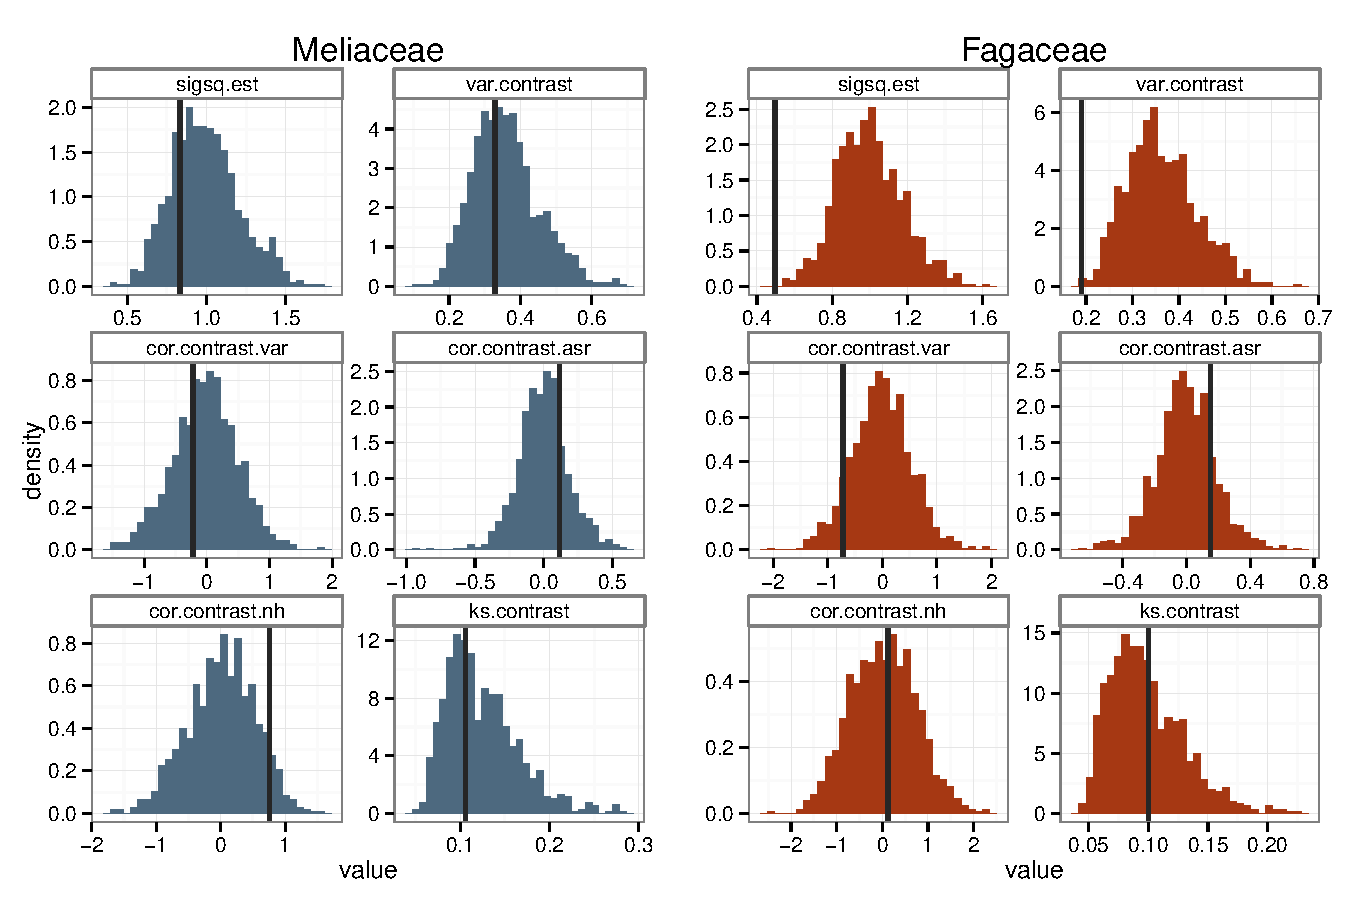
\includegraphics[scale=0.65]{figs/two-clade-example}
  \caption{To be added.}
  \label{fig:two-clades}
\end{figure}

\begin{figure}[p]
  \centering
  \caption{Big fancy tree figure}
  \label{fig:angio-phylogeny}
\end{figure}

\begin{figure}[p]
  \centering
  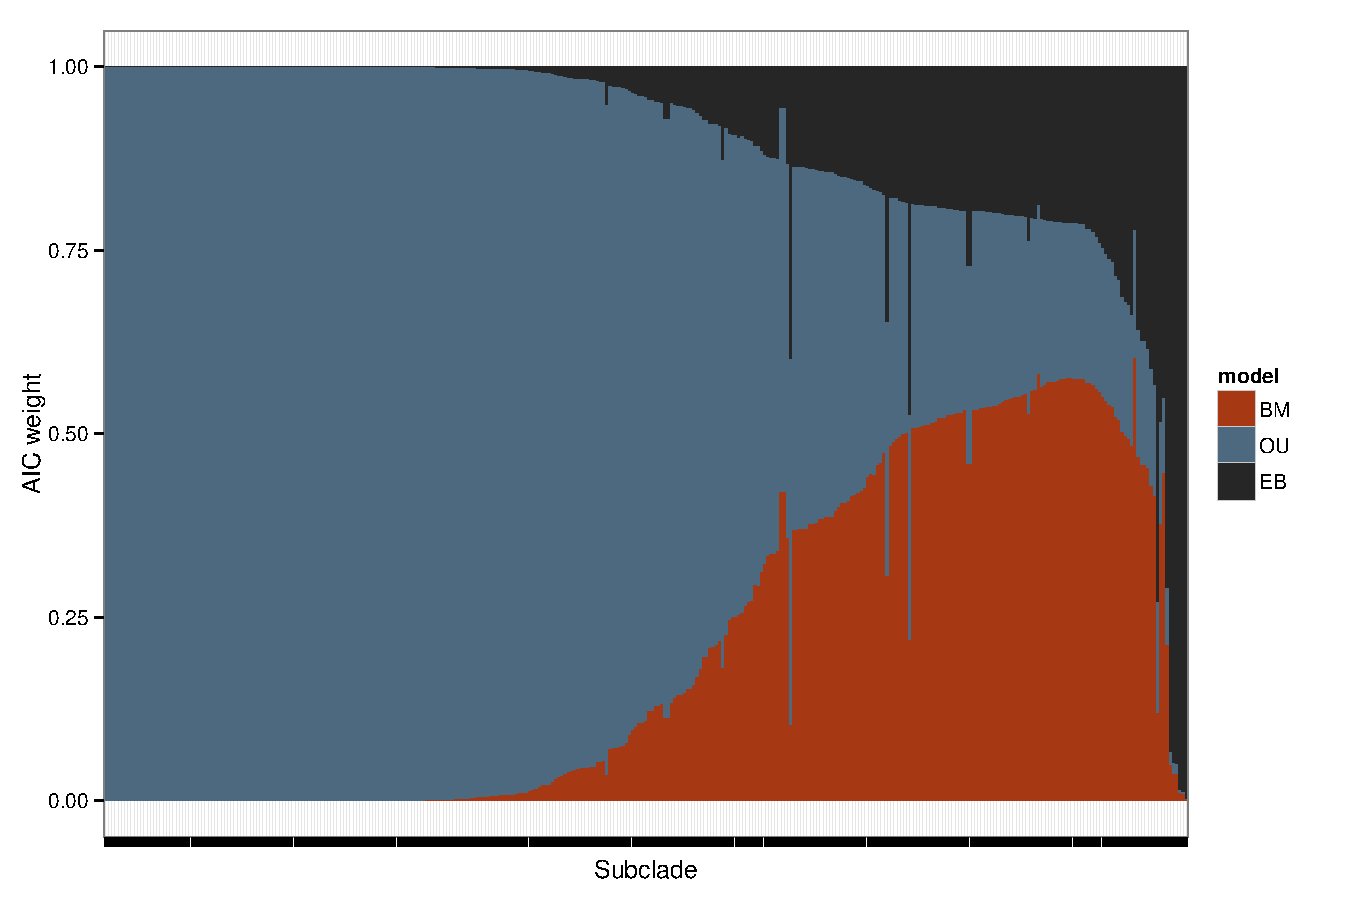
\includegraphics[scale=0.7]{figs/AIC-support}
  \caption{aic support}
  \label{fig:aic-support}
\end{figure}

\begin{figure}[p]
  \centering
  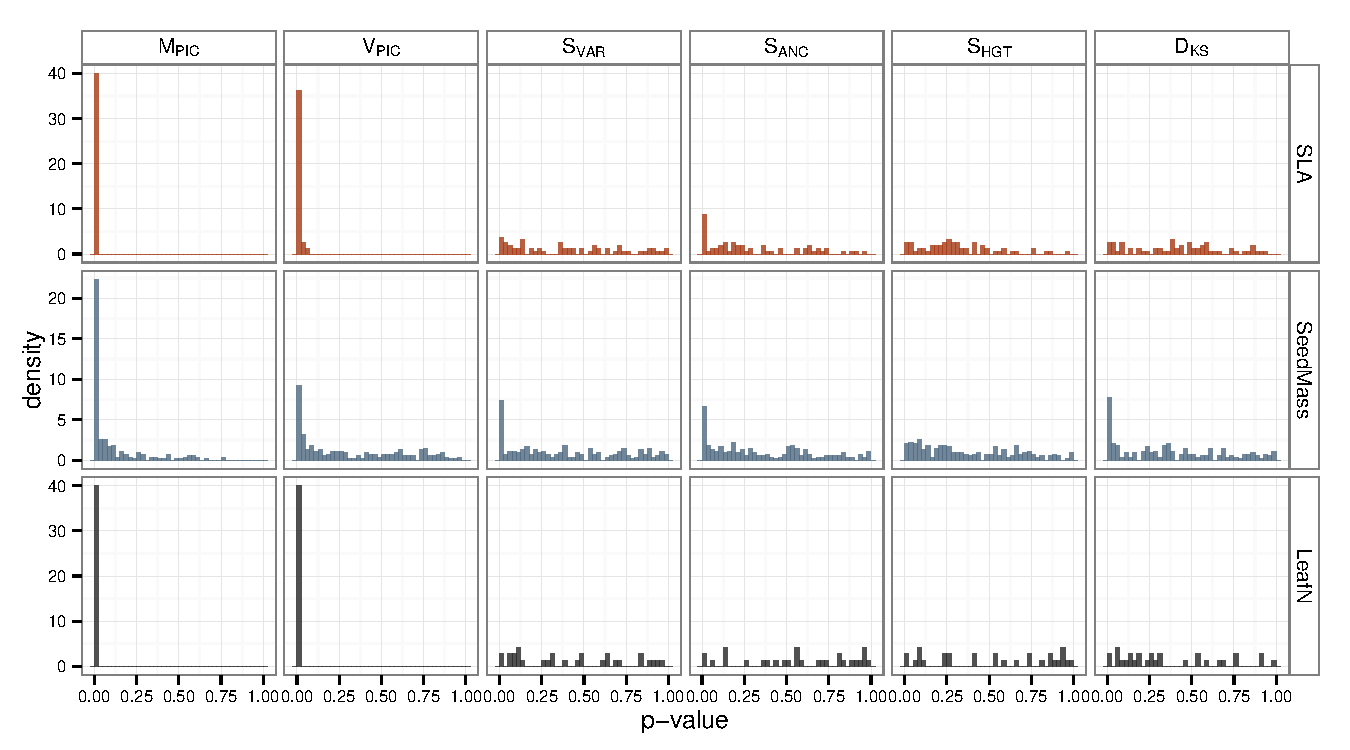
\includegraphics{figs/pvalue-hist-ML}
  \caption{pvalues}
  \label{fig:pvalues}
\end{figure}

\begin{figure}[p]
  \centering
  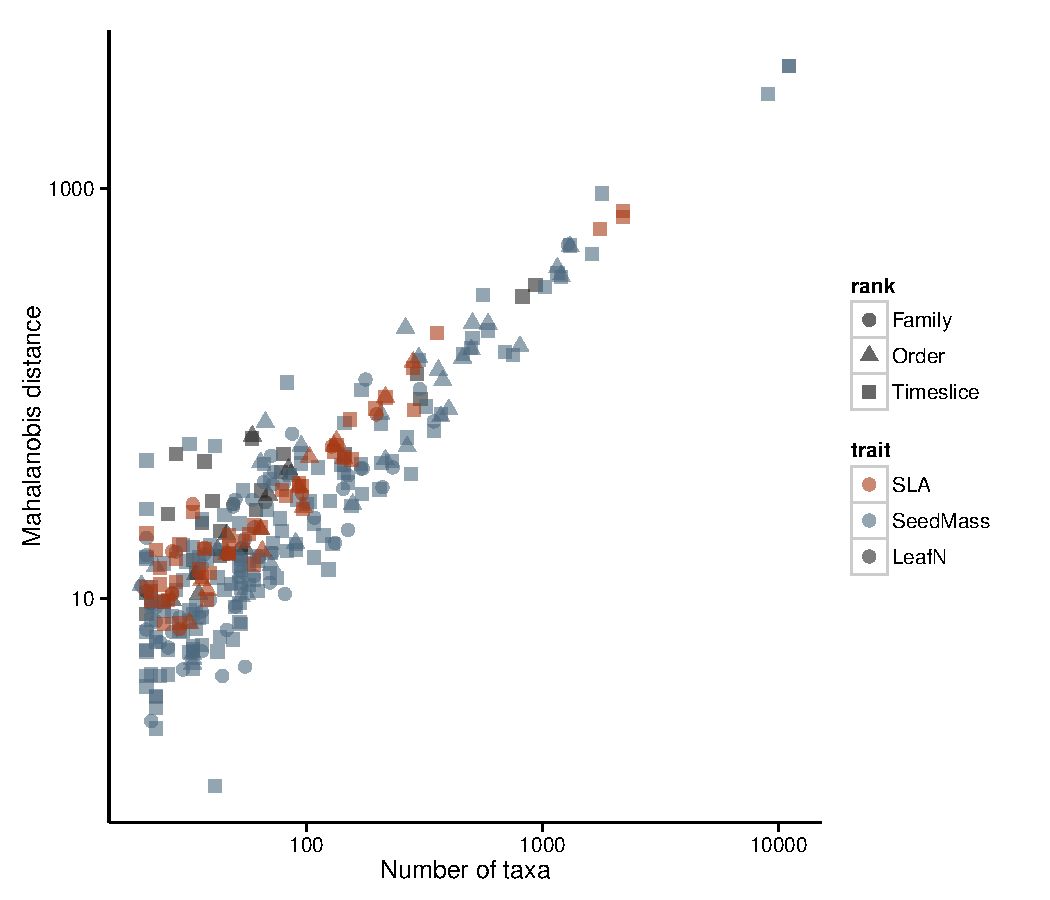
\includegraphics[scale=0.9]{figs/Size-adequacy-ML-bestonly}
  \caption{adequacy v. size}
  \label{fig:size-adequacy}
\end{figure}



\end{document}


